\documentclass[a4paper,11pt]{article}
\usepackage[portuguese]{babel}
\usepackage{graphicx}
\usepackage{amsmath}
\usepackage{enumitem}
\usepackage{fancyvrb}
\usepackage[utf8]{inputenc}
\usepackage[T1]{fontenc}

\usepackage[twoside,verbose,body={16cm,24cm},
left=25mm,top=20mm]{geometry}

\title{Algoritmos e Complexidade\\ Ficha 2: Resolução}

\author{Eduardo Freitas Fernandes}
\date{2025}

\begin{document}
	
	\maketitle
	
	\section{Contagem}
	
	\textbf{Exercício 1}\\
	
	\noindent \textbf{Função \texttt{bubbleSort()}}:\\
	
	\noindent \textbf{Comparações entre elementos do array}:
	O número de comparações entre elementos do array é igual em todos os casos, isto é, o conteúdo do array não altera a execução da função, logo o melhor e pior caso terão o mesmo custo.\\
	\[
		T_{bubbleSort}(N) = \sum_{i=1}^{N-1} \sum_{j=0}^{i-1} 1 = \sum_{i=1}^{N-1} i = \frac{(N-1) \times N}{2} = \Theta(N^2)
	\]
	
	\noindent \textbf{Trocas Efetuadas}:
	\begin{itemize}
		\item \textbf{Melhor caso}: array ordenado por ordem crescente (condição do \texttt{if statement} é sempre falsa)
		\item \textbf{Pior caso}: array ordenado por ordem decrescente (condição do \texttt{if statement} é sempre verdadeira)
	\end{itemize}
	
	\noindent \textbf{Função \texttt{iSort()}}:\\
	
	\noindent \textbf{Comparações entre elementos do array}:
	\begin{itemize}
		\item \textbf{Melhor caso}: array ordenado por ordem crescente (apenas uma comparação no loop interno, de cada iteração do loop externo)
		\[ T_{iSort}(N) = \sum_{i=1}^{N-1} 1 = N-1 = \Omega(N) \]
		\item \textbf{Pior caso}: array ordenado por ordem decrescente
		\[ T_{iSort}(N) = \sum_{i=1}^{N-1} \sum_{j=1}^{i} 1 = \sum_{i=1}^{N-1} i = \frac{N^2 - N}{2} = O(N^2) \]
	\end{itemize}
	
	\noindent Para as trocas de elementos, o melhor e pior caso são os mesmos, dado que o \texttt{swap} depende da condição de paragem do \texttt{for loop}.\\
	
	\newpage
	
	\noindent \textbf{Exercício 2}\\
	
	\noindent Seja N o número de bits necessários para representar \texttt{x}, teremos a seguinte gama de valores:
	\begin{itemize}
		\item $ 2^{N-1} $, que corresponde a todos os bits excepto o mais significativo serem 0 (melhor caso)
		\item $ \sum_{k=0}^{N-1} 2^k = 2^N - 1 $, no caso dos bits serem todos 1 (pior caso)
	\end{itemize}
	
	\noindent \textbf{Função \texttt{mult1()}}:\\
	
	\noindent O número de somas e subtrações é igual, logo não é necessário especificar cada um. O número de operações primitivas (\texttt{+ -}) no \textbf{pior caso} será:
	
	\[ T_{mult1}(N) = 2^N - 1 = \Theta(2^N) \]
	
	\noindent \textbf{Função \texttt{mult2()}}:\\
	
	\noindent No pior caso, todos os bits estão a 1, logo a condição avaliada no \texttt{if statement} será sempre verdadeira, então a operação primitiva \texttt{+} será executada tantas vezes quanto as operações \texttt{\% / *}. Podemos concluir que a complexidade é \textbf{linear}, em função do número de bits, pois a cada iteração um dos bits de \texttt{x} passa a 0 e é efetuada uma adição.\\
	
	
	\noindent \textbf{Exercício 3}
	
	\[
		T(N) = \sum_{i=0}^{N-1} \sum_{j=i}^{N-1} \sum_{k=i}^{j} 1 = \sum_{i=0}^{N-1} \sum_{j=i}^{N-1} j-i+1 = \sum_{i=0}^{N-1} \sum_{j=i}^{N-1} j	
	\]
	\[
		= \sum_{i=0}^{N-1} \frac{(N-i) \times (N-1+i)}{2} = \sum_{i=0}^{N-1} \frac{N^2 + ...}{2} = \frac{N^3}{3} + ... = \Theta(N^3)
	\]
	
	\noindent \textbf{Nota}: na resolução deste somatório decidi remover a expressão $ -i + 1 $ devido ao facto de ser uma constante no segundo somatório, então teria pouco impacto no resultado final da complexidade e iria dificultar os cálculos.
	
\begin{Verbatim}[tabsize=4]
int maxSoma(int v[], int N) {
	int max, i, t;
	int c[N];
	c[0] = v[0];
	max = c[0];
	for (i = 1; i < N; i++) {
		t = c[i - 1] + v[i];
				
		if (t > c[i - 1]) c[i] = t;
		else c[i] = v[i];
				
		if (c[i] > max) max = c[i];
	}
	return max;
}
	\end{Verbatim}
	\[
	T_{maxSoma}(N) = 1 + \sum_{i=1}^{N-1} 2 = 1 + 2 \times (N-1) = \Theta(N)
	\]
	
	
	\noindent \textbf{Exercício 4}\\
	
	\noindent Comparações entre elementos do array:
	
	\begin{itemize}
		\item \textbf{Melhor Caso}: array estritamente decrescente
		\item \textbf{Pior Caso}: array estritamente crescente
	\end{itemize}
	\[
		T_{maxcresc}(N) = \sum_{i=0}^{N-1} \sum_{j=1}^{N-1} 1 = \sum_{i=0}^{N-1} N - 1 = N \times (N-1) = O(N^2)
	\]
	
	\noindent Ao realizar a optimização \texttt{i += m}, serão efetuadas apenas \texttt{N} comparações, pois \texttt{m} terá o valor \texttt{N}, pondo fim ao ciclo. Isto acontece porque o array está ordenado por ordem crescente, então \texttt{m} será o comprimento do maior segmento crescente, que corresponde a \texttt{N}.
	
	
	\section{Definições Recursivas}
	
	\noindent \textbf{Exercício 1}\\
	
	\noindent a)
	
	\begin{figure}[h]
		\centering
		\fbox{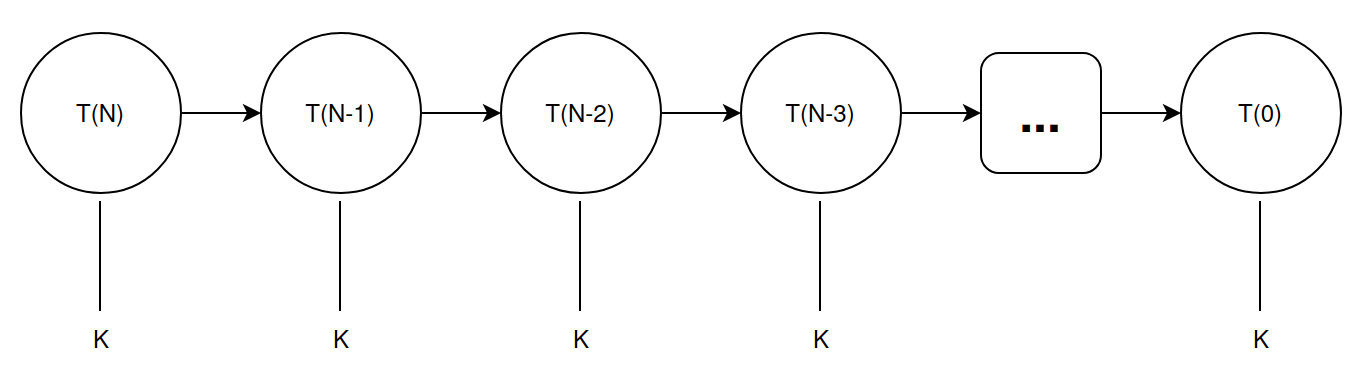
\includegraphics[width=0.8\textwidth]{imgs/2_1-a.png}}
	\end{figure}
	\[
		T(N) = \sum_{i=0}^{N} K = (N + 1) \times K = \Theta(N)
	\]
	
	\noindent b)
	
	\begin{figure}[h]
		\centering
		\fbox{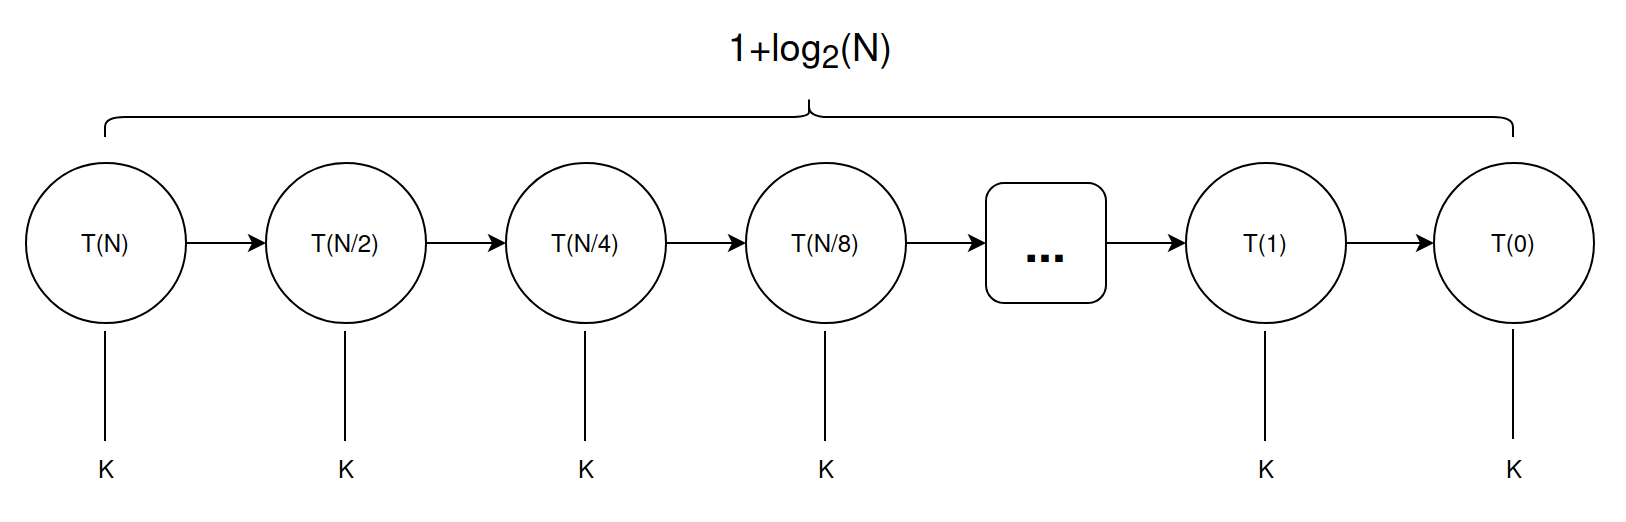
\includegraphics[width=0.8\textwidth]{imgs/2_1-b.png}}
	\end{figure}
	\[
		T(N) = \sum_{i=0}^{1 + \log_2(N)} K = (2 + \log_2(N)) \times K = \Theta(\log_2(N))
	\]
	
	\newpage
	
	\noindent c)
	
	\begin{figure}[h]
		\centering
		\fbox{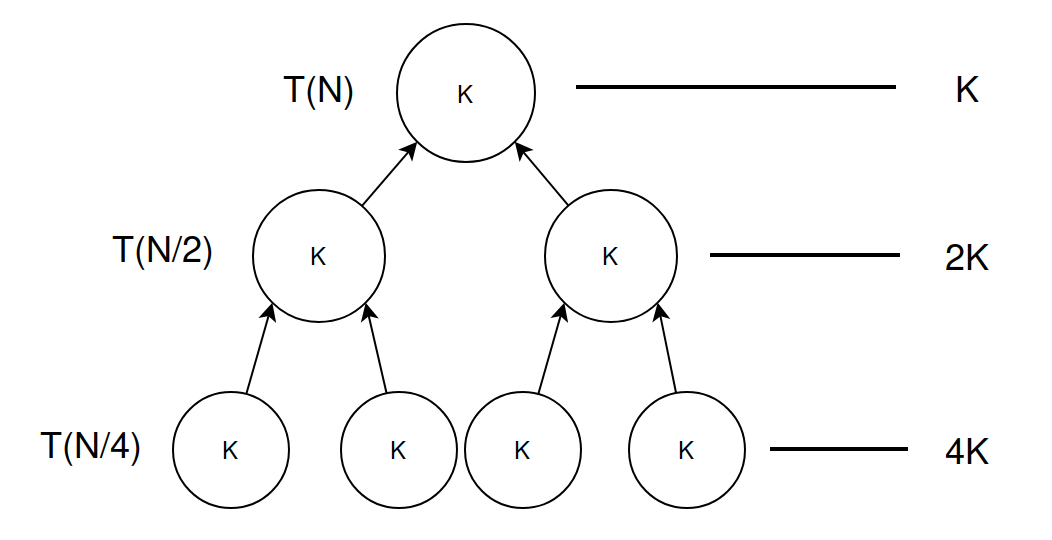
\includegraphics[width=0.6\textwidth]{imgs/2_1-c.png}}
	\end{figure}
	\[
		T(N) = \sum_{i=0}^{1 + \log_2(N)} 2^i \times K = K \times (2^{\log_2(N) + 2} - 1) = K \times (4 \times N - 1) = \Theta(N)
	\]
	
	\noindent d)
	
	\begin{figure}[h]
		\centering
		\fbox{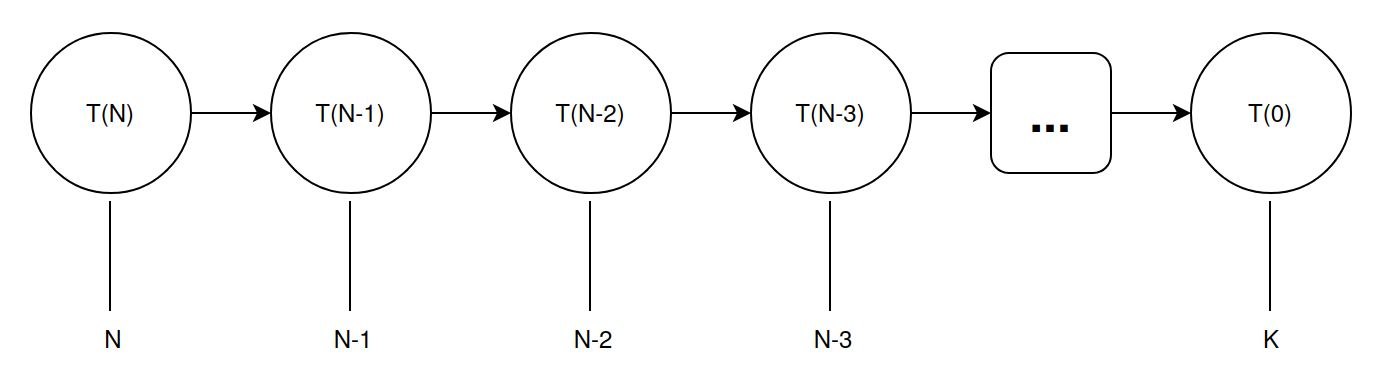
\includegraphics[width=0.8\textwidth]{imgs/2_1-d.png}}
	\end{figure}
	\[
		T(N) = K + \sum_{i=1}^{N} i = K + \frac{N \times (N + 1)}{2} = \Theta(N^2)
	\]
	
	\noindent e)
	
	\begin{figure}[h]
		\centering
		\fbox{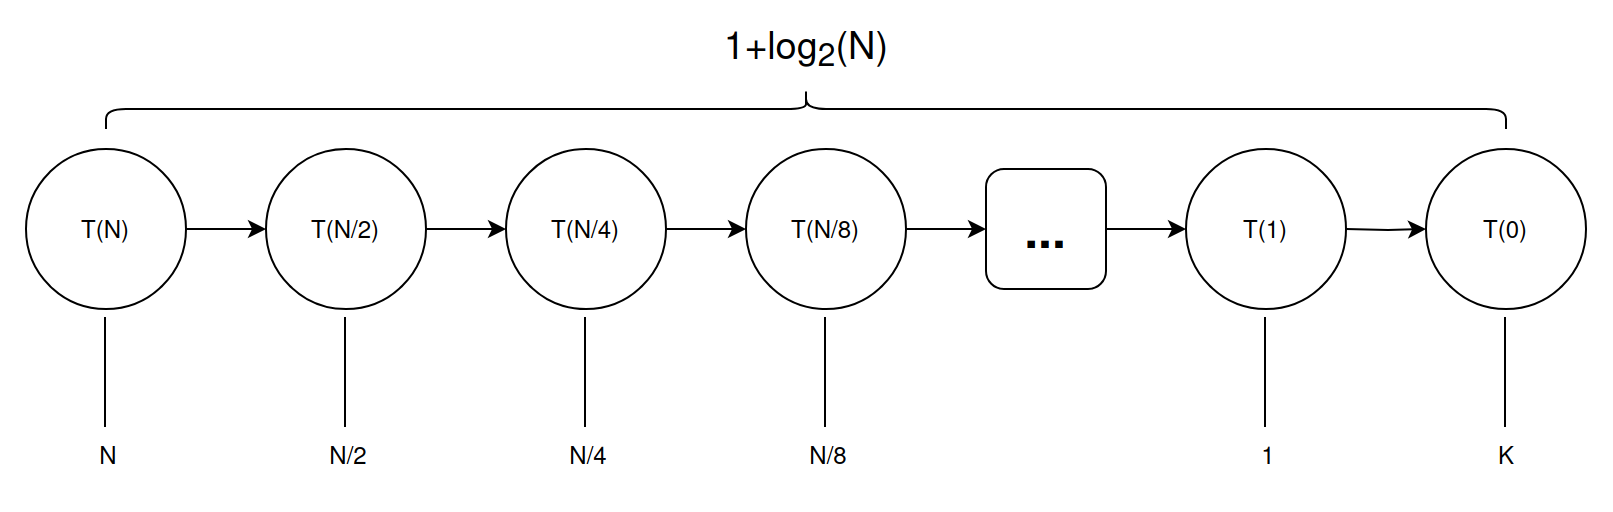
\includegraphics[width=0.8\textwidth]{imgs/2_1-e.png}}
	\end{figure}
	\[
		T(N) = K + \sum_{i=1}^{1 + \log_2(N)} \frac{N}{2^i} = K + 2^{\log_2(N) + 1} - 1 = K + 2 \times N - 1 = \Theta(N)
	\]
	
	\newpage
	
	\noindent f)
	
	\begin{figure}[h]
		\centering
		\fbox{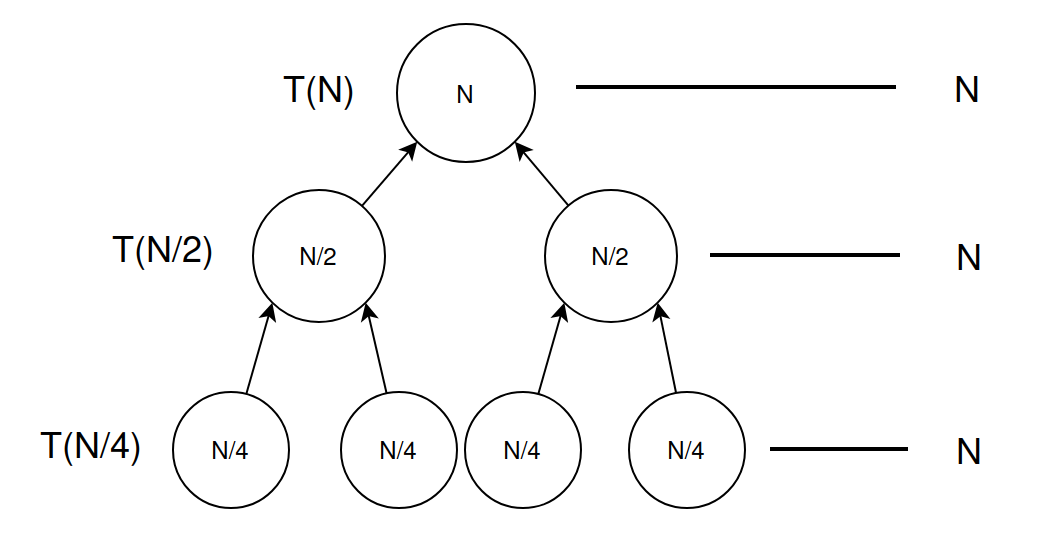
\includegraphics[width=0.6\textwidth]{imgs/2_1-f.png}}
	\end{figure}
	\[
		T(N) = K + \sum_{i=1}^{1 + \log_2(N)} N = K + N \times (1 + \log_2(N)) = \Theta(N \times \log_2(N))
	\]
	
	\noindent \textbf{Exercício 2}
	
	\[
		T(N) =
		\begin{cases}
			0 & N \leq 0 \\
			1 + N - 1 + T(N - 1) & N > 0
		\end{cases}
		\quad = \quad
		\begin{cases}
			0 & N \leq 0 \\
			N + T(N - 1) & N > 0
		\end{cases}
	\]
	\[
		= \sum_{i=1}^{N} i = \frac{N \times (N + 1)}{2} = \Theta(N^2)
	\]
	
	
	\noindent \textbf{Exercício 3}
	
	\[
		T(N) = 
		\begin{cases}
			0 & N \leq 0 \\
			1 + 2 \times T(N - 1) & N > 0
		\end{cases}
	\]
	
	\begin{figure}[h]
		\centering
		\fbox{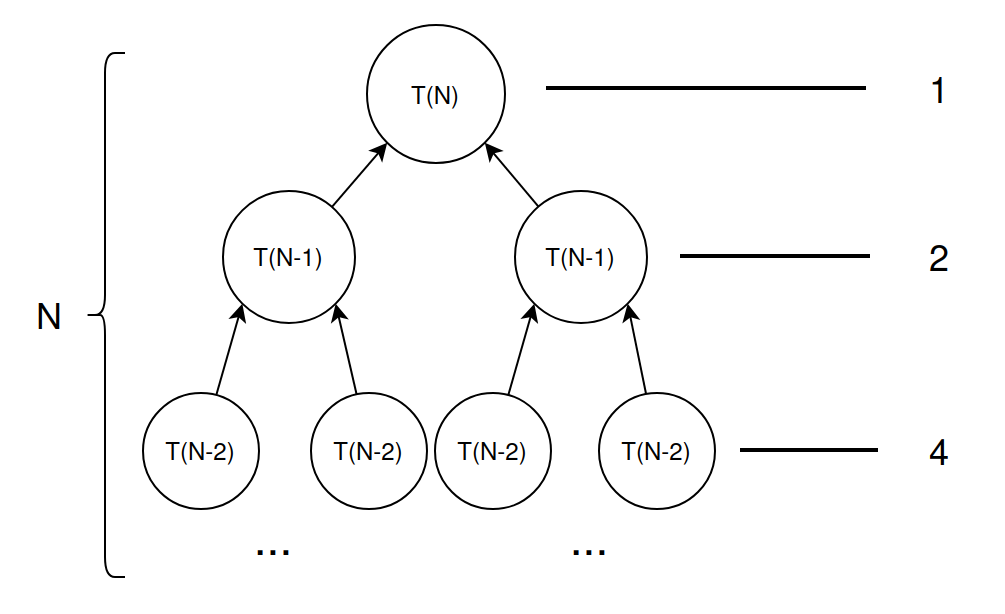
\includegraphics[width=0.7\textwidth]{imgs/2_3.png}}
	\end{figure}
	
	\[
		T(N) = \sum_{i=0}^{N-1} 2^i = 2^N - 1 = \Theta(2^N)
	\]
	
	\newpage
	
	\noindent \textbf{Exercício 4}
	
	\[
		T(N) = 
		\begin{cases}
			1 & N \leq 1 \\
			T_{mergeH}(N) + 2 \times T(N / 2) & N > 1
		\end{cases}
		=
		\begin{cases}
			1 & N \geq 1 \\
			2 \times N + 2 \times T(N/2) & N > 1
		\end{cases}
	\]
	
	\[
		= \sum_{i=1}^{1 + \log_2(N)} 2 \times N = 2 \times N \times (1 + \log_2(N)) = \Theta(N \times \log_2(N))
	\]
	
	\noindent \textbf{Exercício 5}\\
	
	\noindent \textbf{Árvores Equilibradas}
	
	\[
		T(N) = 
		\begin{cases}
			0 & N \leq 0 \\
			1 + 2 \times T(\frac{N-1}{2}) & N > 0
		\end{cases}
		=
		\begin{cases}
			0 & N \leq 0 \\
			1 + 2 \times T(N/2) & N > 0
		\end{cases}
	\]
	\[
		= \sum_{i=0}^{1 + \log_2(N)} 2^i = 4 \times N - 1 = \Theta(N)
	\]
	
	\noindent \textbf{Árvores "Lista"}
	
	\[
	T(N) = 
	\begin{cases}
		0 & N \leq 0 \\
		1 + T(N - 1) & N > 0
	\end{cases}
	\quad = \quad \sum_{i=1}^{N} 1 = N = \Theta(N)
	\]
	
	
	
	\section{Análise de Caso Médio}
	
	\noindent \textbf{Exercício 1}\\
	
	\noindent \textbf{Pior caso}: $ T_{crescente}(N) = \sum_{i=1}^{N} 1 = N - 1 = O(N) $\\
	
	\noindent \textbf{Melhor caso}: $ T_{crescente}(N) = 1 = \Omega(1) $\\
	\[
		T_{crescente}(N) = \Omega(1), O(N)
	\]
	
	\noindent \textbf{Caso médio} da função \texttt{crescente()}:
	
	\[
		\overline{T}_{crescente}(N) = (\sum_{i=1}^{N-1} (\frac{1}{2})^{i-1} \times (1-\frac{1}{2}) \times i) + (\frac{1}{2})^{N-1} \times (N - 1)
	\]
	\[
		\overline{T}(N) = \sum_{i=1}^{N-1} (\frac{1}{2})^i \times i + (\frac{1}{2})^{N-1} \times (N - 1) = \frac{1}{2} + \frac{1}{2} + \frac{3}{8} + \frac{1}{4} + \frac{5}{32} + ... < 2
	\]
	
	\noindent Temos então $ \overline{T}_{crescente}(N) = \Theta(1) $.\\
	
	\noindent \textbf{Caso médio} da função \texttt{maxCresc()}:
	\[
		\overline{T}_{maxCresc}(N) = \sum_{i=0}^{N-1} \overline{T}_{crescente}(N) = \sum_{i=0}^{N-1} 1 = \Theta(N)
	\]
	
	\newpage
	
	\noindent \textbf{Exercício 2}
	
	\noindent \textbf{Exercício 3}\\
	
	\noindent \textbf{Pior caso}: $ T_{strNdif}(N) = \sum_{i=1}^{N} 1 = N - 1 = O(N) $\\
	
	\noindent \textbf{Melhor caso}: $ T_{strNdif}(N) = 1 = \Omega(1) $\\
	\[
	T_{strNdif}(N) = \Omega(1), O(N)
	\]
	
	\noindent \textbf{Caso médio} da função \texttt{strNdif()}:
	\[
	\overline{T}_{strNdif}(N) = (\sum_{i=0}^{N-1} (\frac{1}{26})^{i-1} \times (1-\frac{1}{26}) \times i) + (\frac{1}{26})^{N-1} \times (N - 1)
	\]
	
	
	\noindent \textbf{Exercício 4}\\
	
	\noindent Para calcular o valor esperado do número de bit flips teremos que escrever a soma dos vários casos possíveis, pesados pela respectiva probabilidade. Para isso efectuamos uma contagem dos inputs correspondentes a cada um dos casos:
	
	\begin{itemize}
		\item metade dos bitvectors de comprimento N têm o bit menos significativo a 0;
		\item dos restantes, metade têm o \textbf{segundo} bit menos significativo a 0, i.e. terminam em 01;
		\item dos restantes, metade têm o \textbf{terceiro} bit menos significativo a 0, i.e. terminam em 011;
		\item e assim sucessivamente.
	\end{itemize}
	
	\noindent Temos então:
	
	\[
		\overline{T}(N) = \frac{1}{2} \times 1 flip + \frac{1}{4} \times 2 flips + \frac{1}{8} \times 3 flips + ... + \frac{1}{2^N} \times N + \frac{1}{2^N} \times N
	\]
	
	\noindent Existem duas situações em que ocorrem N bit flips:
	
	\begin{itemize}
		\item todos os bits estão a 1, excepto o mais significativo (0111)
		\item todos os bits estão a 1 (1111)
	\end{itemize}
	\[
		\overline{T}(N) = \sum_{k=1}^{N} \frac{k}{2^k} + \frac{1}{2^N} \times N
	\]
	
	\noindent Uma vez que $ \sum_{k=1}^{\infty} \frac{k}{2^k} = 2 $, temos $ \overline{T}(N) < 2 = \Theta(1) $.\\
	
	\noindent \textbf{Exercício 5}
	
	\noindent \textbf{Exercício 6}\\
	
	\noindent \textbf{Melhor caso}: o array \texttt{a} não contém uma potência de 2, isto é, existe mais do que uma ocorrência do valor 1 no array, ou não existe nenhuma. O custo será $\Theta(N)$.\\
	
	\noindent \textbf{Pior caso}: o array \texttt{a} contém uma potência de 2, isto é, existe apenas uma ocorrência do valor 1 no array. O custo será $\Theta(2^N)$.\\
	
	\section{Análise Amortizada}
	
	\noindent \textbf{Exercício 1}\\
	
	\noindent Análise assimptótica da função \texttt{enqueue()}: a inserção de elementos é sempre feita na stack A, e as operações em stacks são constantes, a função tem sempre o mesmo comportamento seja qual for o input, logo:
	\[
		T_{enqueue}(N) = \Theta(1)
	\]
	
	\noindent Análise assimptótica da função \texttt{dequeue()}:
	\begin{itemize}
		\item \textbf{Melhor caso}: a stack B não está vazia, $ T_{dequeue}(N) = \Omega(1) $.
		\item \textbf{Pior caso}: a stack B está vazia, então remove-se todos os elementos de A e coloca-se em B, $ T_{dequeue}(N) = \sum_{i=1}^{N} 2 = 2 \times N = O(N) $.
	\end{itemize}
	\[
		T_{dequeue}(N) = \Omega(1), O(N)
	\]
	
	\noindent \textbf{Análise Amortizada}:\\
	
	\noindent A \textbf{função de potencial} deve traduzir o trabalho efetuado em cada estado, então iremos usar o número de elementos na stack A como medida:
	\[
		\Phi(Q) = |A|
	\]
	
	\noindent quantos mais elementos em A, maior será o trabalho futuro de os transferir para a stack B.
	\begin{itemize}
		\item $\Phi(Q) \geq 0$, o número de elementos na stack nunca é negativo
		\item $\Phi(Q_0) = 0$, ambas as stacks começam vazias
	\end{itemize}
	
	\noindent Função \texttt{enqueue()}:\\
	
	\noindent O custo real de adicionar um elemento à stack A é constante, indicado no enunciado, logo $c_i = 1$. O potencial no estado $i$ é $|A|+1$, pois a stack A tem mais um elemento, enquanto que $\Phi_{i-1} = |A|$.
	\begin{align*}
		\hat{c}_i & = c_i + \Phi_i - \Phi_{i-1} \\
		\hat{c}_i & = 1 + |A| + 1 - |A| = 2
	\end{align*}
	
	\noindent Logo, podemos concluir que o custo amortizado de cada execução da função \texttt{enqueue()} é \textbf{constante}.\\
	
	\noindent Função \texttt{dequeue()}:\\
	
	\noindent Existem duas situações a analisar nesta função, quando a stack B não está vazia e quando está vazia. Quando a stack B não está vazia, a análise é simples, não há alteração no número de elementos da stack A, por isso a variação de potencial é nula, $\Delta \Phi = 0$, então o custo amortizado será igual ao custo real, que é 1.\\
	
	\noindent Quando a stack B está vazia, todos os elementos de A são passados para B. o custo desta operação é $ 2 |A| + 1 $, dado que é feito um \texttt{pop} e um \texttt{push} a todos os elementos, e por último um \texttt{pop}. O potencial no estado atual é 0, pois a stack A foi esvaziada, e no estado anterior é $|A|$.
	\begin{align*}
		\hat{c}_i & = c_i + \Phi_i + \Phi_{i-1} \\
		\hat{c}_i & = 2 |A| + 1 + 0 - |A| \\
		\hat{c}_i & = |A| + 1
	\end{align*}
		
	\noindent O valor obtido indica que o custo amortizado de \texttt{dequeue()} é linear, mas estamos apenas a considerar uma sequência de operações \texttt{dequeue()}, e não as operações \texttt{enqueue()} que colocaram os elementos na stack A. Tendo isto em conta o custo amortizado é constante, pois o custo de remover todos os elementos de A é amortizado pelo custo de os colocar lá, ou seja, numa única operação o custo é linear, mas foi necessário N iterações da função \texttt{enqueue()}, com um custo constante, para amortizar o custo de \texttt{dequeue()}.\\
	
	\noindent \textbf{Exercício 2}\\
	
	\noindent Seja N o número de elementos na stack, a função de potencial a utilizar será $\Phi(Q) = N$. Existem duas situações a analisar: (1) k é menor que o número de elementos na stack, logo o custo real será k; (2) o número de elementos na stack é menor que k, logo o custo real será N.\\
	
	\noindent (1) No caso de $ k < N $, o custo amortizado será:
	\[
		\hat{c}_i = k + N - k - N = 0
	\]
	
	\noindent O potencial no estado anterior é N, que corresponde ao número de elementos da stack, o potencial no estado atual é $ N - k $, pois foram retirados k elementos à stack.\\
	
	\noindent (2) No de caso de $ k \geq N $, o custo amortizado será:
	\[
		\hat{c}_i = N + 0 - N = 0
	\]
	
	\noindent Neste caso, foram removidos todos os elementos da stack, daí o potencial no estado atual ser 0, pois a stack está vazia. Podemos então concluir que o \textbf{custo amortizado} da função \texttt{multiPop()} é O(1).\\
	
	\noindent \textbf{Exercício 3}\\
	
	\noindent Análise \textbf{assimptótica} da função \texttt{insert\_rem}:
	\begin{itemize}
		\item \textbf{Melhor caso}: inserir \texttt{x} à cabeça da lista, $ T_{insert\_rem}(N) = \Omega(1) $.
		\item \textbf{Pior caso}: inserir \texttt{x} no fim da lista, $ T_{insert\_rem}(N) = \sum_{i=1}^{N} 1 = O(N) $.
	\end{itemize}
	\[
		T_{insert\_rem}(N) = \Omega(1), O(N)
	\]
	
	\noindent Análise \textbf{agregada}:
	
	\begin{center}
	\begin{tabular}{|c|c|c|c|}
		\hline
		i & input & output & $ c_i $ \\
		\hline
		\hline
		1 & & 20 & 1 \\
		2 & 20 & 70 & 2 \\
		3 & 70 & 60 $\rightarrow$ 70 & 1 \\
		4 & 60 $\rightarrow$ 70 & 30 $\rightarrow$ 60 $\rightarrow$ 70 & 1 \\
		5 & 30 $\rightarrow$ 60 $\rightarrow$ 70 & 40 $\rightarrow$ 60 $\rightarrow$ 70 & 2 \\
		6 & 40 $\rightarrow$ 60 $\rightarrow$ 70 & 50 $\rightarrow$ 60 $\rightarrow$ 70 & 2 \\
		7 & 50 $\rightarrow$ 60 $\rightarrow$ 70 & 10 $\rightarrow$ 50 $\rightarrow$ 60 $\rightarrow$ 70 & 1 \\
		8 & 10 $\rightarrow$ 50 $\rightarrow$ 60 $\rightarrow$ 70 & 80 & 5 \\
		... & & & \\
		\hline
	\end{tabular}
	\end{center}
	
	\newpage
	
	\noindent Custo das 8 operações:
	\[
		1 + 2 + 1 + 1 + 2 + 2 + 1 + 5 = 15
	\]
	
	\noindent Custo \textbf{amortizado} por operação:
	\[
		\frac{15}{8} = 1.875
	\]
	
	\noindent Seja N o número de elementos na lista, a função de \textbf{potencial} será a seguinte:
	\[
		\Phi(S) = N
	\]

	\noindent O custo de executar a função \texttt{insert\_rem()} é $ k + 1 $, sendo $k$ o número de elementos removidos e 1 o custo de adicionar. Podemos então calcular o custo amortizado:
	\begin{align*}
		\hat{c}_i & = c_i + \Phi_i - \Phi_{i-1} \\
		\hat{c}_i & = k + 1 + (N - (k + 1)) - N \\
		\hat{c}_i & = 2
	\end{align*}
	
	\noindent Logo, podemos concluir que o custo amortizado de \texttt{insert\_rem()} é \textbf{constante}.
	
	
\end{document}